\documentclass[12pt]{article}

\usepackage{anyfontsize}
\usepackage{enumitem}
\usepackage{physics} 
\usepackage{enumerate}
\usepackage{pgfplots}
\usepackage{pgfplotstable}
\usepackage{tikz,pgfplots}
\usepackage{graphicx}
\usepackage{float} 
\usepackage{subfigure}
\usepackage[toc,page]{appendix}
\usepackage{amsmath}  %I added this so that you can use the align tool for equations!
\usepackage{amssymb}
\usepackage{array}
\usepackage{tabularx}
\usepackage{cellspace}
\usepackage{geometry}
\usepackage{listings}
\usepackage{color}
\usepackage{fontspec}
\usepackage{booktabs}
\usepackage{newtxtext,newtxmath}
\usepackage{caption}

\geometry{
  a4paper,
  total = {170mm, 257mm},
  left = 20mm,
  top = 20mm,
  }

\definecolor{dkgreen}{rgb}{0,0.6,0}
\definecolor{gray}{rgb}{0.5,0.5,0.5}
\definecolor{mauve}{rgb}{0.58,0,0.82}
\lstset{frame = tb,
        language = Python,
        aboveskip = 3mm,
        belowskip = 3mm,
        showstringspaces = False,
        columns = flexible,
        basicstyle = {\small\ttfamily},
        numbers = left,
        numberstyle = \tiny\color{gray},
        keywordstyle = \color{blue},
        commentstyle = \color{dkgreen},
        stringstyle = \color{mauve},
        breaklines = true,
        breakatwhitespace = true,
        tabsize=4}

\renewcommand\lstlistingname{Algorithm}
\captionsetup[lstlisting]{singlelinecheck=false, margin=12pt, labelsep=default, labelfont=default}
%We can also use: labelsep=period or labelsep=spacce, labelfont=default or labelfont=bf
\pgfplotsset{compat = 1.18}


%%%%%%%%%%%%%%%%%%%%%%%%%%%%%%%% Again, Don't change anything Above %%%%%%%%%%%%%%%%%%%%%%%%%%%%%%%%


\begin{document}

\title{\textbf{{\normalsize Computational Physics Lab}\\
                Homework 3}}
\author{108000204\\
        Yuan-Yen Peng\\
        Dept.\ of Physics, NTHU\\
        Hsinchu, Taiwan}
\date{\today}
\maketitle


\section{Programming Assignments}
  \subsection{(1) Normal Cloud}
  In this section, in the beginning, we create a cloud of particles ($N = 10^4$) distributed by a normal distribution with zero mean and one variance (or in other words, $s.d. = 1$) in 3D Cartesian coordinates. Additionally, we set the initial particle velocities, and accelerations are distributed by the same normal distribution and the system's total mass is $20$. We, afterward, use our N body simulation code from t = 0 up to t = 10 with a constant time step $\Delta t = 0.01$ and a soften length $r_{soft} = 0.01$. We, meanwhile, implement {\ttfamily numba @njit} with 8 cores to accelerate the loop speed ({\ttfamily @jit (nopython=True)} have spent more time so I discard to use it). Besides, I, firstly, set the particle's number = $10^5$ tried to use either {\ttfamily @jit} or {\ttfamily @njit} to accelerate the code; however, with {\ttfamily RK4} it takes no lowering than 800 minutes! Therefore, I use $10^4$, instead. Figure\ref{RK4_cloud} is the group of snap-shot of the normal cloud distribution with the RK4 method and with the extended boundary from -50 to +50. This is a time-consuming task, for orders of 4, RK4, it took 42015 [s]; for orders of two, RK2 and Leapfrog, they took 29506 and 18009 [s], respectively. The last order of one, Euler, took 17794 [s].
  
  \vspace{6pt}

  \begin{figure}[H]
    \centering 
    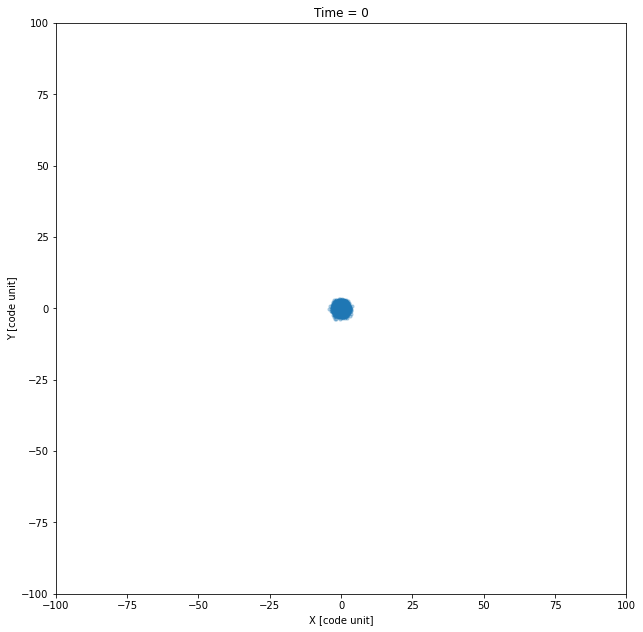
\includegraphics[width = 0.45\textwidth]{./RK4/RK4_0.png}
    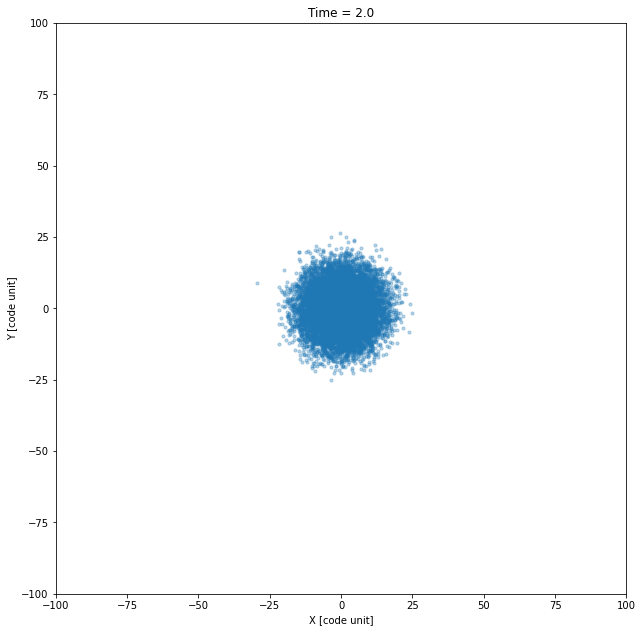
\includegraphics[width = 0.45\textwidth]{./RK4/RK4_2.png}
  \end{figure}
  \begin{figure}[H]
    \centering 
    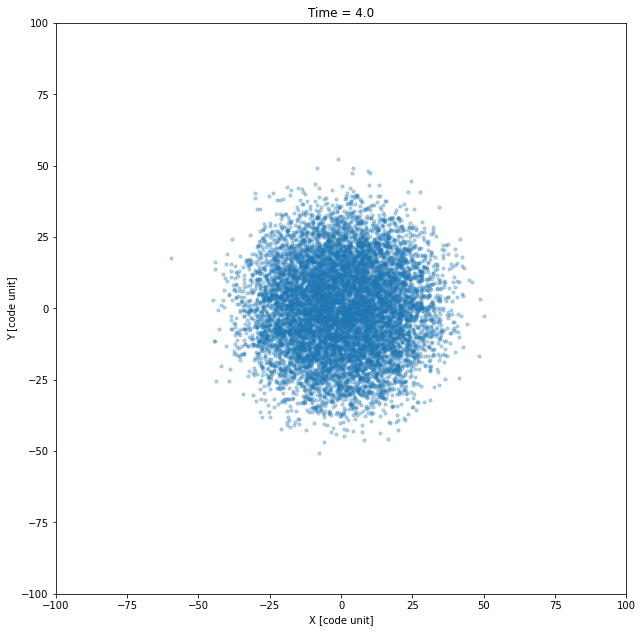
\includegraphics[width = 0.45\textwidth]{./RK4/RK4_4.png} 
    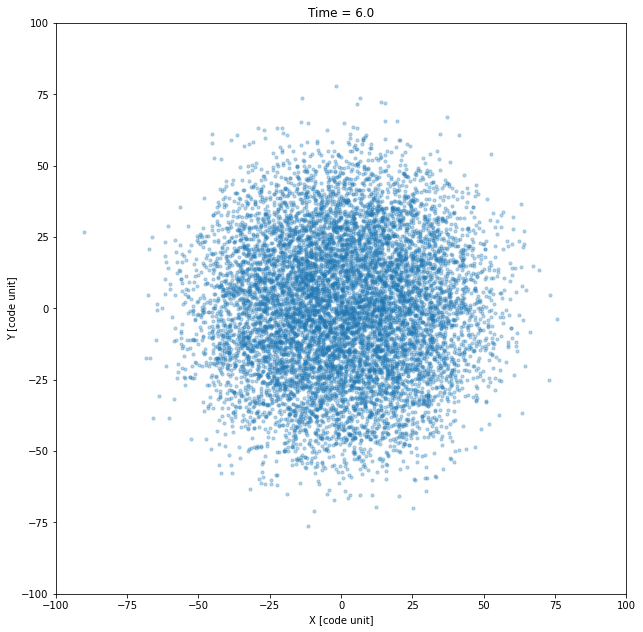
\includegraphics[width = 0.45\textwidth]{./RK4/RK4_6.png}
    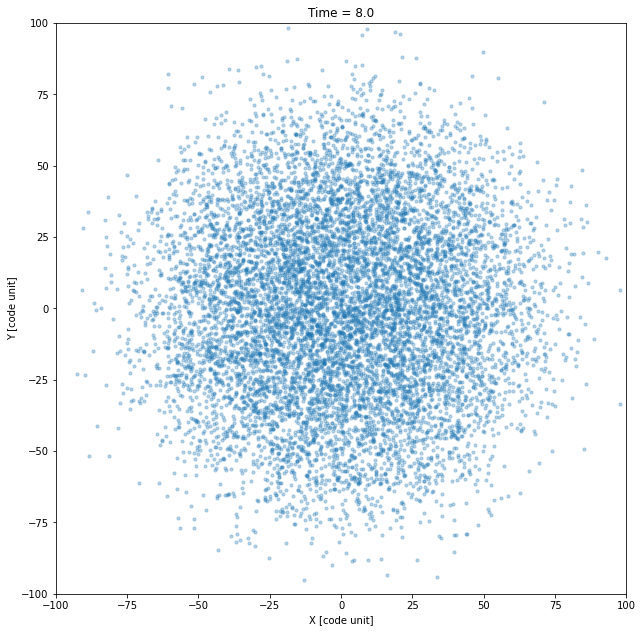
\includegraphics[width = 0.45\textwidth]{./RK4/RK4_8.png}
    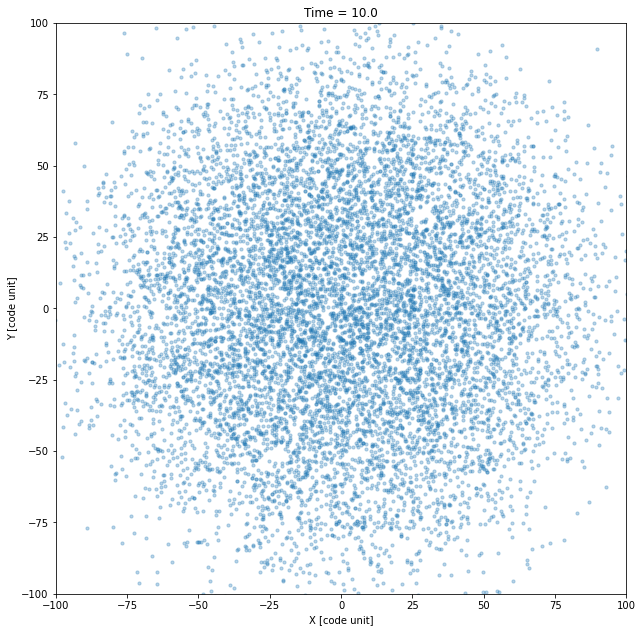
\includegraphics[width = 0.45\textwidth]{./RK4/RK4_10.png} 
    \caption{This the normal cloud with RK4, from $t=0$ to $t=10$ and $dt=0.01$. One run took: 18009 [s]}
    \label{RK4_cloud}
  \end{figure}

  \subsection{(2) Leapfrog method}
  The leapfrog method is a second-order method for solving an initial value problem. The main idea in this is divided into three parts, kick-drift-kick. For each time step $dt$, each particle receives a half-step kick,
  \[v_{i+1/2} = v_i + a_i\frac{dt}{2}\]
  and use the above half-step velocity, and followed by a full-step drift,
  \[x_{i+1} = x_i + v_{i+1/2}dt\]
  and lastly, use the above drift, and followed by another half-step kick,
  \[v_{i+1} = v_{i+1/2} + a_{i+1}\frac{dt}{2}\]
  \newline
  In the next subsection, we will discuss and compare the Leapfrog method with Euler, RK2, and RK4 as well.

  \begin{figure}[H]
    \centering 
    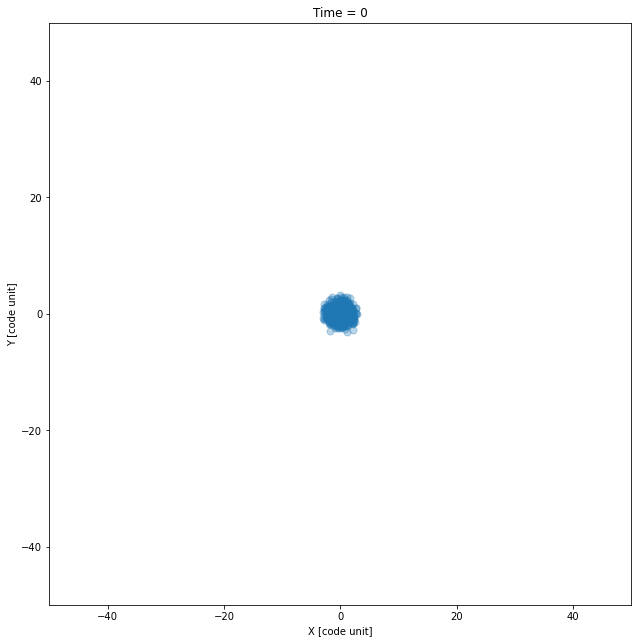
\includegraphics[width = 0.45\textwidth]{./LF/0.png} 
    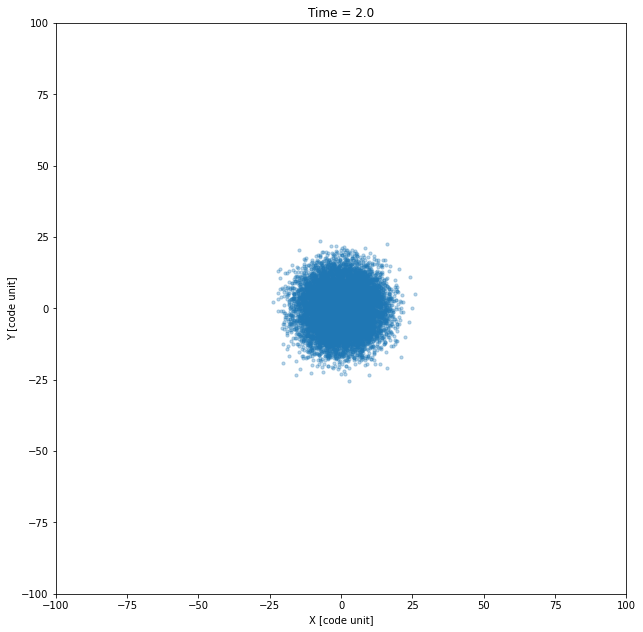
\includegraphics[width = 0.45\textwidth]{./LF/2.png} 
    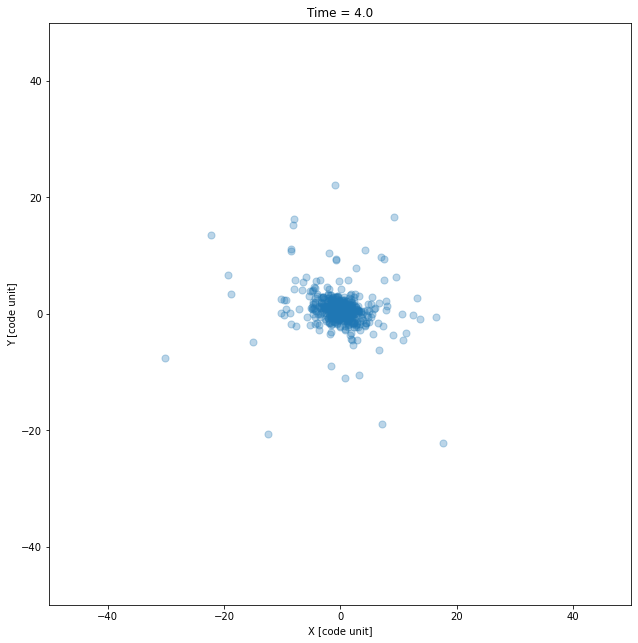
\includegraphics[width = 0.45\textwidth]{./LF/4.png} 
    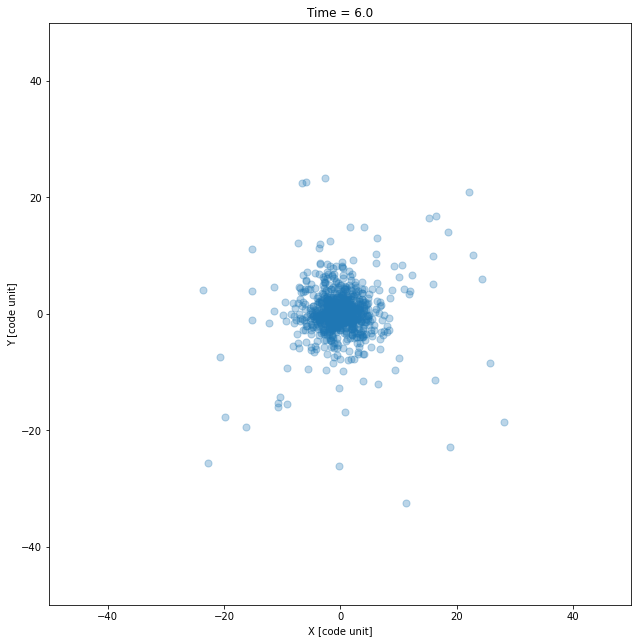
\includegraphics[width = 0.45\textwidth]{./LF/6.png} 
    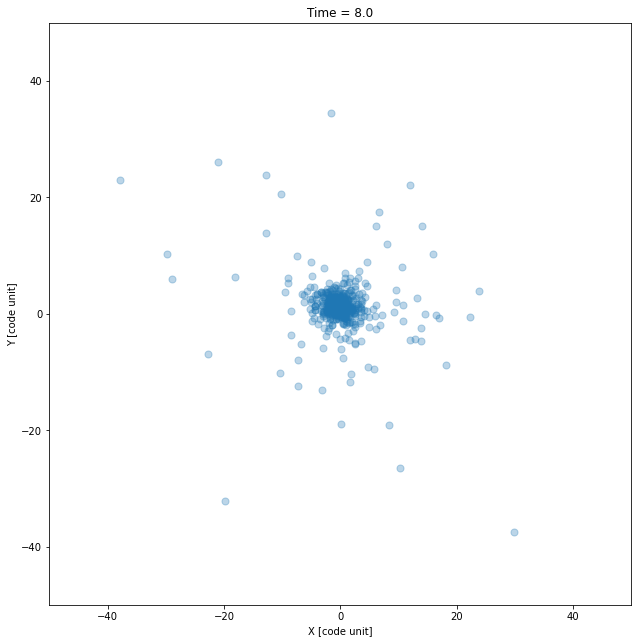
\includegraphics[width = 0.45\textwidth]{./LF/8.png} 
    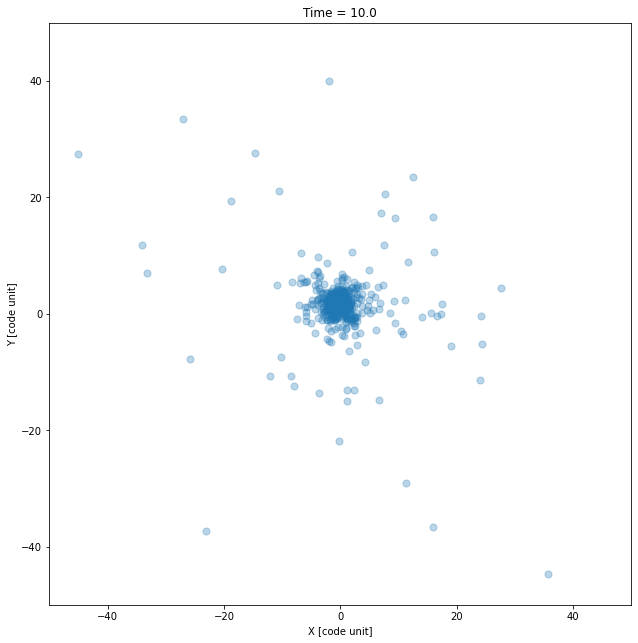
\includegraphics[width = 0.45\textwidth]{./LF/10.png}  
    \caption{This the normal cloud with Leapfrog, from $t=0$ to $t=10$ and $dt=0.01$. One run took: 18009 [s]}
    \label{LF}
  \end{figure}

  \subsection{(3) Energy comparison}
  In this section, we will discuss kinetic energy, potential energy, and total energy. The definitions are below:
  \[U = -\frac{Gm_{i}m_{j}}{r + r_{soft}}\]
  \[K = \frac{1}{2}m_{i}v_{i}^{2}\]
  \[E = U + K\]
  where the subscriptions indicate which particles; $G$ is the gravitational constant, here we set it to 1; $m$ is the mass of each particle; $r$ and $r_{soft}$ is the distance between two particles and the tolerance of distance, which can avoid the nominator equal to zero. After defining all the parameters, we use four different methods, Euler, RK2, RK4, and Leapfrog, and implement the initial conditions as in section 1 to rerun the codes.
  \newline

  See in Figure \ref{E1}\textasciitilde\ref{E4}, we can find out that the potential energy is much smaller than the kinetic energy owing to the small masses of particles. On the other hand, the total energy is dominated by the kinetic part, which makes sense to us. In Figure \ref{E1}\textasciitilde\ref{E4}, we can also see the total energy is not the ``constant'' at the beginning because we initially set the normal random accelerations to each particle which can be regarded that there are other forces applied to the particles. Nevertheless, in the wake of a little period, the total energy will gradually be in a stable stage because of no external force. These phenomena not merely can see in the Euler but in others as well. Compare this with the stable speed, which means how long to be stable. We use RK4 as the theoretical benchmark. It is obvious that Euler (first order) is the slowest one; in the other words, it is the most distorted one; for the second order, RK2 is shapeless at the beginning, and Leapfrog is the most similar one with the benchmark. Therefore, we can conclude that if individuals want to calculate a large number of particles problem, they can choose the Leapfrog method because it has not merely high speed but also high accuracy. (detail of accuracy can see in the next section, the accuracy compared with the benchmark is within one order.)

  \begin{figure}[H]
    \centering 
    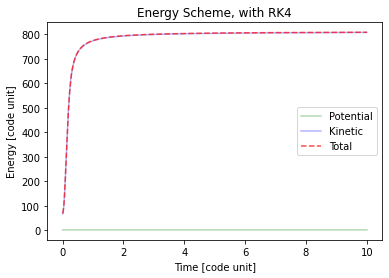
\includegraphics[width = 10cm]{RK4_E.png}
    \caption{RK4, y-axis is Energy; x-axis is time.}
    \label{E1}
  \end{figure}

  \begin{figure}[H]
    \centering 
    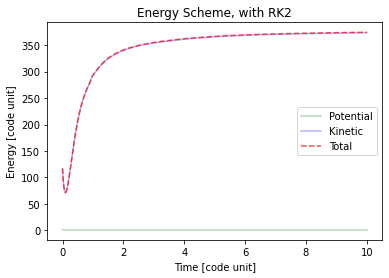
\includegraphics[width = 10cm]{RK2_E.png}
    \caption{RK2, y-axis is Energy; x-axis is time.}
    \label{E2}
  \end{figure}

  \begin{figure}[H]
    \centering 
    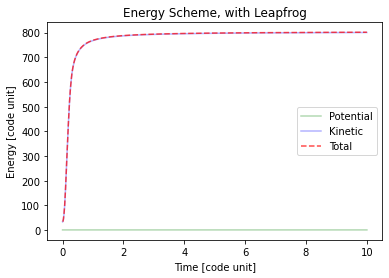
\includegraphics[width = 10cm]{LF_E.png}
    \caption{Leapfrog, y-axis is Energy; x-axis is time.}
    \label{E3}
  \end{figure}

  \begin{figure}[H]
    \centering 
    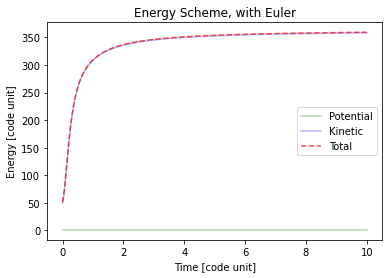
\includegraphics[width = 10cm]{Euler_E.png}
    \caption{Euler, y-axis is Energy; x-axis is time.}
    \label{E4}
  \end{figure}

  So as to analyze the accuracy of the Leapfrog method, we set the RK4 (fourth order) as a benchmark. We, likewise, applied a logarithm of 10 to investigate the order of accuracy thereafter. In Figure \ref{RK4_LF}, we can see the accuracy comparisons between Leapfrog methods and the benchmark.

  \begin{figure}[H]
    \centering 
    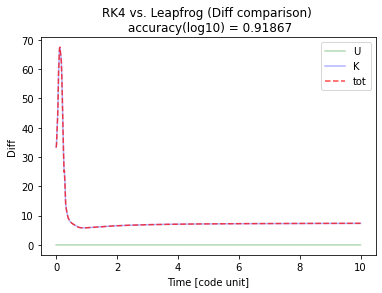
\includegraphics[width = 10cm]{RK4_D.png}
    \caption{In the comparison of energy schemes between the RK4 and Leapfrog methods, the average accuracy is approximately 0.9 orders.}
    \label{RK4_LF}
  \end{figure}


\section{Codes}
    All the codes are transferred from jupyterlab or python codes; hence, if you want to re-run them, please see the source code in the attached files or my GitHub repository: \newline
    {\centerline{\ttfamily <https://github.com/gary20000915/Comphyslab-HW3.git>}}

    \subsection{{\ttfamily\ particles.py}}
      \begin{lstlisting}[language={Python}]
import numpy as np

class Particles:
    """
    
    The Particles class handle all particle properties

    for the N-body simulation. 

    """
    def __init__(self, N:int = 100):
        """
        Prepare memories for N particles

        :param N: number of particles.

        By default: particle properties include:
                nparticles: int. number of particles
                _masses: (N,1) mass of each particle
                _positions:  (N,3) x,y,z positions of each particle
                _velocities:  (N,3) vx, vy, vz velocities of each particle
                _accelerations:  (N,3) ax, ay, az accelerations of each partciel
                _tags:  (N)   tag of each particle
                _time: float. the simulation time 

        """
        self.nparticles = N
        self._time = 0 # initial time = 0
        self._masses = np.ones((N, 1))
        self._positions = np.zeros((N, 3))
        self._velocities = np.zeros((N, 3))
        self._accelerations = np.zeros((N, 3))
        self._tags = np.linspace(1, N, N)
        self._U = np.ones((N, 1))
        self._K = np.ones((N, 1))
        
        return


    def get_time(self):
        return self._time
    
    def get_masses(self):
        return self._masses
    
    def get_positions(self):
        return self._positions
    
    def get_velocities(self):
        return self._velocities
    
    def get_accelerations(self):
        return self._accelerations
    
    def get_tags(self):
        return self._tags
    
    def get_time(self):
        return self._time
    
    def get_U(self):
        return self._U
    
    def get_K(self):
        return self._K


    def set_time(self, time):
        self._time = time
        return
    
    def set_masses(self, mass):
        self._masses = mass
        return
    
    def set_positions(self, pos):
        self._positions = pos
        return
    
    def set_velocities(self, vel):
        self._velocities = vel
        return
    
    def set_accelerations(self, acc):
        self._accelerations = acc
        return
    
    def set_tags(self, IDs):
        self._tags = IDs
        return
    
    def set_U(self, U):
        self._U = U
        return
    
    def set_K(self, K):
        self._K = K
        return
    
    def output(self, fn, time):
        """
        Write simulation data into a file named "fn"
        """
        mass = self._masses
        pos  = self._positions
        vel  = self._velocities
        acc  = self._accelerations
        tag  = self._tags
        header = """
                ----------------------------------------------------
                Data from a 3D direct N-body simulation. 

                rows are i-particle; 
                coumns are :mass, tag, x ,y, z, vx, vy, vz, ax, ay, az

                NTHU, Computational Physics Lab

                ----------------------------------------------------
                """
        header += "Time = {}".format(time)
        np.savetxt(fn,(tag[:],mass[:,0],pos[:,0],pos[:,1],pos[:,2],
                            vel[:,0],vel[:,1],vel[:,2],
                            acc[:,0],acc[:,1],acc[:,2]),header=header)

        return
      \end{lstlisting}
      
    \subsection{{\ttfamily\ simulation.py}}
      \begin{lstlisting}[language={Python}]
import numpy as np
from pathlib import Path
import time
from numba import jit, njit, prange, set_num_threads
from nbody.particles import Particles 
import matplotlib.pyplot as plt

"""

This program solve 3D direct N-particles simulations 
under gravitational forces. 

This file contains two classes:

1) Particles: describes the particle properties
2) NbodySimulation: describes the simulation

Usage:

    Step 1: import necessary classes

    from nbody import Particles, NbodySimulation

    Step 2: Write your own initialization function

    
        def initialize(particles:Particles):
            ....
            ....
            particles.set_masses(mass)
            particles.set_positions(pos)
            particles.set_velocities(vel)
            particles.set_accelerations(acc)

            return particles

    Step 3: Initialize your particles.

        particles = Particles(N=100)
        initialize(particles)


    Step 4: Initial, setup and start the simulation

        simulation = Simulation(particles)
        simulation.setip(...)
        simulation.evolve(dt=0.001, tmax=10)


Author: Yuan-Yen Peng (editted from Prof. Kuo-Chuan Pan, NTHU 2022.10.30)
Dept. of Physics, NTHU
Date: Npv. 28, 2022
For the course, computational physics lab

"""

def ACC_norm(N, posx, posy, posz, G, mass, rsoft, U, K, vel_square):
    '''
    Acceleration with normal for loops.
    
    :param N: number of particles
    :param posx: position x
    :param posy: position y
    :param posz: position z
    :param G: gravitational constant
    :param mass: mass
    '''
    
    acc = np.zeros((N, 3))
    for i in range(N):
        for j in range(N):
            if j > i:
                x = posx[i] - posx[j]
                y = posy[i] - posy[j]
                z = posz[i] - posz[j]
                r = np.sqrt(x**2 + y**2 + z**2) + rsoft
                theta = np.arccos(z / r)
                phi = np.arctan2(y, x)
                F = - G * mass[i, 0] * mass[j, 0] / np.square(r)
                Fx = F * np.cos(theta) * np.cos(phi)
                Fy = F * np.cos(theta) * np.sin(phi)
                Fz = F * np.sin(theta)

                acc[i, 0] += Fx / mass[i, 0]
                acc[j, 0] -= Fx / mass[j, 0]

                acc[i, 1] += Fy / mass[i, 0]
                acc[j, 1] -= Fy / mass[j, 0]
                
                acc[i, 2] += Fz / mass[i, 0]
                acc[j, 2] -= Fz / mass[j, 0]
                
                U[i] = -G * mass[i, 0] * mass[j, 0] / r
                K[i] = 0.5 * (mass[i, 0] * np.sum(vel_square[i, :]) 
                              + mass[j, 0] * np.sum(vel_square[j, :]))
    return acc, U, K

@jit(nopython=True)
def ACC_jit(N, posx, posy, posz, G, mass, rsoft, U, K, vel_square):
    '''
    Acceleration with numba jit for loops
    
    :param N: number of particles
    :param posx: position x
    :param posy: position y
    :param posz: position z
    :param G: gravitational constant
    :param mass: mass
    '''
    acc = np.zeros((N, 3))
    for i in range(N):
        for j in range(N):
            if j > i:
                x = posx[i] - posx[j]
                y = posy[i] - posy[j]
                z = posz[i] - posz[j]
                r = np.sqrt(x**2 + y**2 + z**2) + rsoft
                theta = np.arccos(z / r)
                phi = np.arctan2(y, x)
                F = - G * mass[i, 0] * mass[j, 0] / np.square(r)
                Fx = F * np.cos(theta) * np.cos(phi)
                Fy = F * np.cos(theta) * np.sin(phi)
                Fz = F * np.sin(theta)

                acc[i, 0] += Fx / mass[i, 0]
                acc[j, 0] -= Fx / mass[j, 0]

                acc[i, 1] += Fy / mass[i, 0]
                acc[j, 1] -= Fy / mass[j, 0]
                
                acc[i, 2] += Fz / mass[i, 0]
                acc[j, 2] -= Fz / mass[j, 0]
                
                U[i] = -G * mass[i, 0] * mass[j, 0] / r
                K[i] = 0.5 * (mass[i, 0] * np.sum(vel_square[i, :]) 
                              + mass[j, 0] * np.sum(vel_square[j, :]))
    return acc, U, K

set_num_threads(8)
@njit(parallel=True)
def ACC_njit(N, posx, posy, posz, G, mass, rsoft, U, K, vel_square):
    '''
    Acceleration with numba njit for loops (parallel)
    
    :param N: number of particles
    :param posx: position x
    :param posy: position y
    :param posz: position z
    :param G: gravitational constant
    :param mass: mass
    '''
    acc = np.zeros((N, 3))
    for i in prange(N):
        for j in prange(N):
            if j > i:
                x = posx[i] - posx[j]
                y = posy[i] - posy[j]
                z = posz[i] - posz[j]
                r = np.sqrt(x**2 + y**2 + z**2) + rsoft
                theta = np.arccos(z / r)
                phi = np.arctan2(y, x)
                F = - G * mass[i, 0] * mass[j, 0] / np.square(r)
                Fx = F * np.cos(theta) * np.cos(phi)
                Fy = F * np.cos(theta) * np.sin(phi)
                Fz = F * np.sin(theta)

                acc[i, 0] += Fx / mass[i, 0]
                acc[j, 0] -= Fx / mass[j, 0]

                acc[i, 1] += Fy / mass[i, 0]
                acc[j, 1] -= Fy / mass[j, 0]
                
                acc[i, 2] += Fz / mass[i, 0]
                acc[j, 2] -= Fz / mass[j, 0]
                
                U[i] = - G * mass[i, 0] * mass[j, 0] / r
                K[i] = 0.5 * (mass[i, 0] * np.sum(vel_square[i, :]) 
                              + mass[j, 0] * np.sum(vel_square[j, :]))
    return acc, U, K

class NbodySimulation:
    """
    
    The N-body Simulation class.
    
    """
    
    def __init__(self,particles:Particles):
        """
        Initialize the N-body simulation with given Particles.

        :param particles: A Particles class.  
        
        """

        # store the particle information
        self.nparticles = particles.nparticles
        self.particles  = particles

        # Store physical information
        self.time  = 0.0  # simulation time

        # Set the default numerical schemes and parameters
        self.setup()
        
        return

    def setup(self, G=1, 
                    rsoft=0.01, 
                    method="RK2", 
                    io_freq=10, 
                    io_title="particles",
                    io_screen=True,
                    visualized=False):
        """
        Customize the simulation enviroments.

        :param G: the graivtational constant
        :param rsoft: float, a soften length
        :param meothd: string, the numerical scheme
                       support "Euler", "RK2", and "RK4"

        :param io_freq: int, the frequency to outupt data.
                        io_freq <=0 for no output. 
        :param io_title: the output header
        :param io_screen: print message on screen or not.
        :param visualized: on the fly visualization or not. 
        
        """
        # TODO:
        self.G = G
        self.rsoft = rsoft
        self.method = method
        self.io_freq = io_freq
        self.io_title = io_title
        self.io_screen = io_screen
        self.visualized = visualized
        return

    def evolve(self, dt:float=0.01, tmax:float=1):
        """

        Start to evolve the system

        :param dt: time step
        :param tmax: the finial time
        
        """
        # TODO:
        method = self.method
        if method=="Euler":
            _update_particles = self._update_particles_euler
        elif method=="RK2":
            _update_particles = self._update_particles_rk2
        elif method=="RK4":
            _update_particles = self._update_particles_rk4   
        elif method=="Leapfrog":
            _update_particles = self._update_particles_lf
        else:
            print("No such update meothd", method)
            quit() 

        # prepare an output folder for lateron output
        io_folder = "data_"+self.io_title
        Path(io_folder).mkdir(parents=True, exist_ok=True)
        io_folder_fig = "fig_" + self.io_title
        Path(io_folder_fig).mkdir(parents=True, exist_ok=True)
        
        # ====================================================
        #
        # The main loop of the simulation
        #
        # =====================================================

        # TODO:
        particles = self.particles # call the class: Particles
        n = 0
        t = self.particles.get_time()
        t1 = time.time()
        step = int(tmax / dt) + 1
        UU = np.ones((step, 1))
        KK = np.ones((step, 1))
        EE = np.ones((step, 1))
        for i in range(step):
            # update particles
            particles = _update_particles(dt, particles)[0]
            UU[i] = _update_particles(dt, particles)[1]
            KK[i] = _update_particles(dt, particles)[2]
            EE[i] = UU[i] + KK[i]
            # update io
            if (n % self.io_freq == 0):
                if self.io_screen:
                    # print('n = ', n, 'time = ', t, 'dt = ', dt)
                    # output
                    fn = io_folder+"/data_"+self.io_title+"_"+str(n).zfill(5)+".txt"
                    print(fn)
                    self.particles.output(fn, t)

                    # savefig
                    scale = 100
                    fig, ax = plt.subplots()
                    fig.set_size_inches(10.5, 10.5, forward=True)
                    fig.set_dpi(72)
                    ax.set_xlim(-1*scale,1*scale)
                    ax.set_ylim(-1*scale,1*scale)
                    ax.set_aspect('equal')
                    ax.set_xlabel('X [code unit]')
                    ax.set_ylabel('Y [code unit]')
                    pos = particles.get_positions()
                    plt.title(f'Time = {np.round(t, 0)}')
                    FIG = f'{io_folder_fig}/fig_{self.io_title}_{str(int(0.01 * n)).zfill(1)}.png'
                    ax.scatter(pos[:, 0], pos[:, 1], s = 10, alpha = .3)
                    plt.savefig(FIG)
                    plt.show()
            
            # update time
            if t + dt > tmax:
                dt = tmax - t
            t += dt
            n += 1
        
        T = np.linspace(0, tmax, step)
        plt.plot(T, UU, 'g', alpha = .3, label = 'Potential')
        plt.plot(T, KK, 'b', alpha = .3, label = 'Kinetic')
        plt.plot(T, EE, '--r', alpha = .7, label = 'Total')
        plt.xlabel('Time [code unit]')
        plt.ylabel('Energy [code unit]')
        plt.title(f'Energy Scheme, with {method}')
        plt.legend()
        plt.show()
        t2 = time.time()
        print("Time diff: ", t2 - t1)
        print("Done!")
        
        return [UU, KK]

    def _calculate_acceleration(self, mass, pos):
        """
        Calculate the acceleration.
        """
        # TODO:
        particles = self.particles
        G = self.G
        rsoft = self.rsoft
        posx = pos[:, 0]
        posy = pos[:, 1]
        posz = pos[:, 2]
        N = self.nparticles
        U = particles.get_U()
        K = particles.get_K()
        vel_square = np.square(particles.get_velocities())
        # return ACC_jit(N, posx, posy, posz, G, mass,rsoft, U, K, vel_square)
        return ACC_njit(N, posx, posy, posz, G, mass, rsoft, U, K, vel_square)

    def _update_particles_euler(self, dt, particles:Particles):
        # TODO:
        mass = particles.get_masses()
        pos = particles.get_positions()
        vel = particles.get_velocities()
        acc = self._calculate_acceleration(mass, pos)[0]
        y0 = np.array([pos, vel])
        yder = np.array([vel, acc])
        
        y0 = np.add(y0, yder * dt)
        
        U = np.sum(self._calculate_acceleration(mass, y0[0])[1])
        K = np.sum(self._calculate_acceleration(mass, y0[0])[2])
        
        particles.set_positions(y0[0])
        particles.set_velocities(y0[1])
        particles.set_accelerations(acc)
        
        return particles, U, K

    def _update_particles_rk2(self, dt, particles:Particles):
        # TODO:
        mass = particles.get_masses()
        pos = particles.get_positions()
        vel = particles.get_velocities()
        acc = self._calculate_acceleration(mass, pos)[0]
        
        y0 = np.array([pos, vel])
        yder = np.array([vel, acc])
        k1 = yder
        y_temp = y0 + dt * k1 
        acc = self._calculate_acceleration(mass, y_temp[0])[0]
        k2 = np.array([y_temp[1], acc])
        y0 = np.add(y0, (dt / 2) * (k1 + k2))
        
        acel = self._calculate_acceleration(mass, y0[0])[0]
        U = np.sum(self._calculate_acceleration(mass, y0[0])[1])
        K = np.sum(self._calculate_acceleration(mass, y0[0])[2])
        
        particles.set_positions(y0[0])
        particles.set_velocities(y0[1])
        particles.set_accelerations(acel)
        return particles, U, K

    def _update_particles_rk4(self, dt, particles:Particles):
        # TODO:
        mass = particles.get_masses()
        pos = particles.get_positions()
        vel = particles.get_velocities()
        acc = self._calculate_acceleration(mass, pos)[0]
        
        y0 = np.array([pos, vel])
        yder = np.array([vel, acc])
        k1 = yder
        y_temp = y0 + 0.5 * dt * k1 
        acc = self._calculate_acceleration(mass, y_temp[0])[0]
        k2 = np.array([y_temp[1], acc])
        y_temp = y0 + 0.5 * dt * k2
        acc = self._calculate_acceleration(mass, y_temp[0])[0]
        k3 = np.array([y_temp[1], acc])
        y_temp = y0 + dt * k3
        acc = self._calculate_acceleration(mass, y_temp[0])[0]
        k4 = np.array([y_temp[1], acc])
        
        y0 = np.add(y0, (1/6) * dt * (k1 + 2*k2 + 2*k3 + k4))
        
        acel = self._calculate_acceleration(mass, y0[0])[0]
        U = np.sum(self._calculate_acceleration(mass, y0[0])[1])
        K = np.sum(self._calculate_acceleration(mass, y0[0])[2])
        
        particles.set_positions(y0[0])
        particles.set_velocities(y0[1])
        particles.set_accelerations(acel)
        return particles, U, K
    
    def _update_particles_lf(self, dt, particles:Particles):
        # TODO:
        mass = particles.get_masses()
        pos = particles.get_positions()
        vel = particles.get_velocities()
        
        acc = particles.get_accelerations()
        vel_prime = vel + acc * 0.5 * dt
        pos = pos + vel_prime * dt
        acc = self._calculate_acceleration(mass, pos)[0]
        vel = vel_prime + acc * 0.5 * dt
        
        U = np.sum(self._calculate_acceleration(mass, pos)[1])
        K = np.sum(self._calculate_acceleration(mass, pos)[2])
        
        particles.set_positions(pos)
        particles.set_velocities(vel)
        particles.set_accelerations(acc)
        return particles, U, K


if __name__=='__main__':

    # test Particles() here
    particles = Particles(N=10)
    # test NbodySimulation(particles) here
    sim = NbodySimulation(particles=particles)
    sim.setup(G = 6.67e-8, io_freq=2, io_screen=True, io_title="test")
    sim.evolve(dt = 1, tmax = 10)
    print(sim.G)
    print("Done")
      \end{lstlisting}

    \subsection{{\ttfamily\ NormalCloud.ipynb}}
      \begin{lstlisting}[language={Python}]
# %% [markdown]
# ## Homework 3
# ### Programming Assignment 1
# ### 111 Computational Physics Lab  
#   >Author: Yuan-Yen Peng 108000204  
#   >Email: garyphys0915@gapp.nthu.edu.com  
#   >Date: Nov. 11, 2022  
#   >LICENCE: MIT

# %%
import numpy as np
import glob
from numba import jit, njit, prange, set_num_threads
import matplotlib.pyplot as plt
from mpl_toolkits.mplot3d import Axes3D
import matplotlib.animation as animation
from nbody.particles import Particles
from nbody.simulation import NbodySimulation

# %%
problem_name = "NormalCloud"
Num = int(1e4)
tmax = 10
dt = 0.01
r_soft = 0.001

# %%
set_num_threads(8)
@njit(parallel = True)
def generator(N, positions, velocities, accelerations):
        mu, sigma = 0, 1 # mean = 0; variance = 1, i.e., standard deviation = sqrt(var) = 1
        for i in prange(N):
            positions[i] = np.random.normal(mu, sigma, 3)
            velocities[i] = np.random.normal(mu, sigma, 3)
            accelerations[i] = np.random.normal(mu, sigma, 3)
            
        return [positions, velocities, accelerations]

# %%
def initialRandomParticles(N):
        """
        Initial particles

        """
        total_mass = 20
        particles = Particles(N = N)
        
        positions = particles.get_positions()
        velocities = particles.get_velocities()
        accelerations = particles.get_accelerations()
        masses = particles.get_masses() # ones array (size = N)
        mass = total_mass / particles.nparticles # single particel's mass
        
        particles.set_masses((masses * mass))
        particles.set_positions(generator(N, positions, velocities, accelerations)[0])
        particles.set_velocities(generator(N, positions, velocities, accelerations)[1])
        particles.set_accelerations(generator(N, positions, velocities, accelerations)[2])

        return particles

# %% [markdown]
# solve with t = 0 ~ 10 with dt = 0.01 and r_soft = 0.01.

# %%
# Initial particles here.
method = "RK4"
particles = initialRandomParticles(N = Num)
# Run the n-body simulations
sim = NbodySimulation(particles)
sim.setup(G=1,method=method,io_freq=200,io_title=problem_name,io_screen=True,visualized=False)
Energy_RK4 = sim.evolve(dt=dt,tmax=tmax)

# %%
# Initial particles here.
method = "RK2"
particles = initialRandomParticles(N = Num)
# Run the n-body simulations
sim = NbodySimulation(particles)
sim.setup(G=1,method=method,io_freq=200,io_title=problem_name,io_screen=True,visualized=False)
Energy_RK2 = sim.evolve(dt=dt,tmax=tmax)

# %%
# Initial particles here.
method = "Euler"
particles = initialRandomParticles(N = Num)
# Run the n-body simulations
sim = NbodySimulation(particles)
sim.setup(G=1,method=method,io_freq=200,io_title=problem_name,io_screen=True,visualized=False)
Energy_Euler = sim.evolve(dt=dt,tmax=tmax)

# %%
# Initial particles here.
method = "Leapfrog"
particles = initialRandomParticles(N = Num)
# Run the n-body simulations
sim = NbodySimulation(particles)
sim.setup(G=1,method=method,io_freq=200,io_title=problem_name,io_screen=True,visualized=False)
Energy_LF = sim.evolve(dt=dt,tmax=tmax)

# %%
TT = len(Energy_RK4[0])
Time = np.linspace(0, tmax, len(Energy_RK4[0]))
Diff_tot = np.abs((Energy_RK4[0] + Energy_RK4[1]) - (Energy_LF[0] + Energy_LF[1]))
Diff = np.abs(np.array(Energy_RK4) - np.array(Energy_LF))
avg = np.average(Diff_tot)
accuracy = np.log10(avg)
print("Average = ", avg)
print("Accuracy (log) = ", accuracy)

plt.plot(Time, Diff[0], "g", alpha = .3, label = "U")
plt.plot(Time, Diff[1], "b", alpha = .3, label = "K")
plt.plot(Time, Diff_tot, "--r", alpha = .7, label = "tot")
plt.xlabel("Time [code unit]")
plt.ylabel("Diff")
plt.title(f"RK4 vs. Leapfrog (Diff comparison) \n accuracy(log10) = {np.round(accuracy, 5)}")
plt.legend()
plt.show()

# %%
Energy_RK4 = Energy_RK2
TT = len(Energy_RK4[0])
Time = np.linspace(0, tmax, len(Energy_RK4[0]))
Diff_tot = np.abs((Energy_RK4[0] + Energy_RK4[1]) - (Energy_LF[0] + Energy_LF[1]))
Diff = np.abs(np.array(Energy_RK4) - np.array(Energy_LF))
avg = np.average(Diff_tot)
accuracy = np.log10(avg)
print("Average = ", avg)
print("Accuracy (log) = ", accuracy)

plt.plot(Time, Diff[0], "g", alpha = .3, label = "U")
plt.plot(Time, Diff[1], "b", alpha = .3, label = "K")
plt.plot(Time, Diff_tot, "--r", alpha = .7, label = "tot")
plt.xlabel("Time [code unit]")
plt.ylabel("Diff")
plt.title(f"RK2 vs. Leapfrog (Diff comparison) \n accuracy(log10) = {np.round(accuracy, 5)}")
plt.legend()
plt.show()

# %%
Energy_RK4 = Energy_Euler
TT = len(Energy_RK4[0])
Time = np.linspace(0, tmax, len(Energy_RK4[0]))
Diff_tot = np.abs((Energy_RK4[0] + Energy_RK4[1]) - (Energy_LF[0] + Energy_LF[1]))
Diff = np.abs(np.array(Energy_RK4) - np.array(Energy_LF))
avg = np.average(Diff_tot)
accuracy = np.log10(avg)
print("Average = ", avg)
print("Accuracy (log) = ", accuracy)

plt.plot(Time, Diff[0], "g", alpha = .3, label = "U")
plt.plot(Time, Diff[1], "b", alpha = .3, label = "K")
plt.plot(Time, Diff_tot, "--r", alpha = .7, label = "tot")
plt.xlabel("Time [code unit]")
plt.ylabel("Diff")
plt.title(f"Euler vs. Leapfrog (Diff comparison) \n accuracy(log10) = {np.round(accuracy, 5)}")
plt.legend()
plt.show()



      \end{lstlisting}


\end{document}